\section{Training des Modells}\label{sec:training_modells}

Das Training eines neuronalen Netzes bietet eine Vielzahl an Anknüpfungspunkten, um die Vertraulichkeit der Daten zu sichern.
Der für das Training leichteste Fall ist es, wenn bereits bei der Vorverarbeitung der Daten ein Mechanismus angewendet wurde, der die Vertraulichkeit schützt.
Dies sorgt dafür, dass das Training ohne Anpassung stattfinden kann.
Alternative Methoden, welche im Folgenden detailliert erläutert werden, beeinflussen die Algorithmen der Trainingsmethodik, verändern die Architektur des Modells oder verschlüsseln das gesamte Modell.


\subsection{Training mit Differential Privacy}\label{sec:dp_training}

Nachdem Kapitel \ref{sec:dp} bereits zeigt, wie Differential Privacy definiert wird und bei der Vorverarbeitung von Daten genutzt werden kann, behandelt das folgende Kapitel, wie Differential Privacy während des Trainings genutzt werden kann.

Abadi et al. \cite{P-28} zeigen, wie der Trainingsalgorithmus angepasst wird, um Differential Privacy zu unterstützen.
Die Methode trägt den Namen Differentially private SGD oder auch DPSGD.
Ein Trainingsschritt mittels DPSGD sieht dabei wie folgt aus:
\begin{compactenum}
    \item Ein Batch von zufälligen Daten wird als Input des Modells für den Feedforward Schritt genutzt. Dabei kommt jeder Datenpunkt mit der gleichen Wahrscheinlichkeit in einem Batch vor. Anders als bei einem normalen Training könnten einzelne Datensätze auch mehrmals oder gar nicht innerhalb einer Epoche zum Trainieren genutzt werden. 
    \item Die Gradienten werden mittels der Verlustfunktion berechnet. Dies gleicht dem Training ohne Differential Privacy.
    \item Die maximale Größe der Gradienten wird beschränkt. Dies liegt daran, dass Gradienten potenziell beliebig groß werden könnten, was dafür sorgen könnte, dass das berechnete Privacy Budget nicht eingehalten werden könnte.
    \item Anschließend werden die Gradienten durch den Gauß-Mechanismus verrauscht. 
    \item Die Anpassung der Gewichte erfolgt in die umgekehrte Richtung der Gradienten, skaliert mit einer Lernrate. Dies gleicht ebenfalls dem normalen Trainingsvorgehen.
\end{compactenum}

Ein wichtiger Teil der Methode ist jedoch die Berechnung des $\epsilon$-Werts und des $\delta$-Werts über den Trainingsprozess hinweg.
Hierbei wird für jeden Batch berechnet, welchen Einfluss dieser über die Gradienten auf die Gewichte des Modells hat.
Das Rauschen in Schritt 4 wird dabei so gewählt, dass eine Anpassung der Gewichte durch einen Batch ($\epsilon$,$\delta$)-Differential Privacy erfüllt.
Dadurch, dass ein Batch aus zufälligen Datenpunkten des Datensatzes besteht, kann das sogenannte Privacy Amplification Theorem genutzt werden \cite{P-107}. 
Dieses besagt, dass jede Anpassung in Bezug auf den ganzen Datenbestand ($\mathcal{O}(q\epsilon)$,$q\delta$)-Differential Privacy erfüllt, wobei $q$ dem Strichprobenverhältnis von Batch Größe zu Datensatzgröße entspricht und $\mathcal{O}$ dabei der Big-$\mathcal{O}$-Notation.
Die Big-$\mathcal{O}$-Notation zeigt hier, dass das Privacy Budget höchstens so schnell wächst, wie das Stichprobenverhältnis $q$ mit dem $\epsilon$-Wert eines Batches.
Um nun mehrere Trainingsschritte zu bewerten, könnte das Privacy Budgets eines Schritts mit der Anzahl der Schritte $T$ multipliziert werden. 
Dadurch erfüllt der Trainingsprozess ($\mathcal{O}(q\epsilon T)$,$q\delta T$)-Differential Privacy.

Bei der beschriebene Berechnung des Privacy Budgets, handelt es sich um eine Obergrenze, welche mathematisch bewiesen werden kann.
Es ist jedoch vorteilhaft, eine beweisbare Obergrenze zu finden, welche möglichst nahe an dem tatsächlichen Wert liegt. 
Dies sorgt dafür, dass mehr Rauschen eingefügt werden kann, jedoch die Quantifizierung des Privacy Budgets den gleichen Wert annimmt, was wiederum die tatsächliche Privatsphäre der Daten mehr schützt.
Eine Möglichkeit die Distanz der berechneten Obergrenze bei DPSGD zu minimieren, ist das Strong Composition Theorem \cite{P-27}.
Dabei handelt es sich um ein Theorem, welches dafür sorgt, dass das Privacy Budget über mehrere Schritte geringer ansteigt, primär dadurch, dass nicht mehr mit der Anzahl der Schritte $T$ multipliziert werden muss, sondern nur mit der Wurzel davon.
Formell erfüllt der Trainingsprozess ($\mathcal{O}(q\epsilon \sqrt{T log(1/\delta)})$,$q\delta T$)-Differential Privacy.

Abadi et al. \cite{P-28} zeigen jedoch, dass die Obergrenze sogar noch geringer gesetzt werden kann, als mit dem Strong Composition Theorem.
Diese Methode wird Moment Berechnung genannt und sorgt dafür, dass der Trainingsprozess mit DPSGD ($\mathcal{O}(q\epsilon \sqrt{T})$,$\delta$)-Differential Privacy erfüllt.
Da $\delta$ normalerweise kleiner gesetzt wird, als die Inverse der Anzahl an Datensätzen im Datenbestand, sorgt das Wegfallen des Terms $\sqrt{log (1/\delta)}$ im $\epsilon$-Teil, für eine signifikante Verkleinerung des Privacy Budgets über den Trainingsprozess hinweg.
Zusätzlich entfällt im $\delta$-Teil der Faktor $qT$, wodurch der gesetzte $\delta$-Wert über den Trainingsprozess konstant bleibt.
\subsection{Private Aggregation of Teacher Ensembles PATE}\label{sec:pate}
\subsection{Homomorphe Verschlüsselung}\label{sec:homomorphe_verschlüsselung}

Homomorphe Verschlüsselung ist eine Methodik, um Berechnung auf verschlüsselten Daten durchführen zu können. Dadurch können Daten beispielsweise in der Cloud verarbeitet werden, ohne dass es dem Anbieter des Services möglich ist, die Vertraulichkeit der Daten zu gefährden.

Ein Homomorphismus in der Algebra bezeichnet eine strukturerhaltende Abbildung einer Mengen $G$ in eine andere Menge $H$.
Dabei hat jedes Element $g \in G $ mindestens ein Bild $h \in H$ und die Relationen der Elemente $g \in G$ zueinander, finden sich auch in H wieder \cite{B-2}.

Ein typisches Beispiel ist der Homomorphismus zwischen zwei Gruppen $(G,\circ)$ und $(H,\ast)$, wobei $\circ$ und $\ast$ jeweils eine Verknüpfung innerhalb der Gruppe symbolisieren. 
Die Beziehung der beiden Gruppen wird Gruppenhomomorphismus genannt, wenn es eine Funktion $f:G\to H$ gibt, die Elemente der Gruppe $G$ auf die Gruppe $H$ abbildet und dabei für alle Elemente $g_1,g_2 \in G$ gilt \cite{P-98}:
\begin{equation*}
    f(g_1 \circ g_2) = f(g_1) \ast f(g_2)
\end{equation*}
Abbildung \ref{fig:group_homomorphismus} zeigt eine grafische Darstellung dieses Gruppenhomomorphismus.

\begin{figure}[!htb]
    \centering
    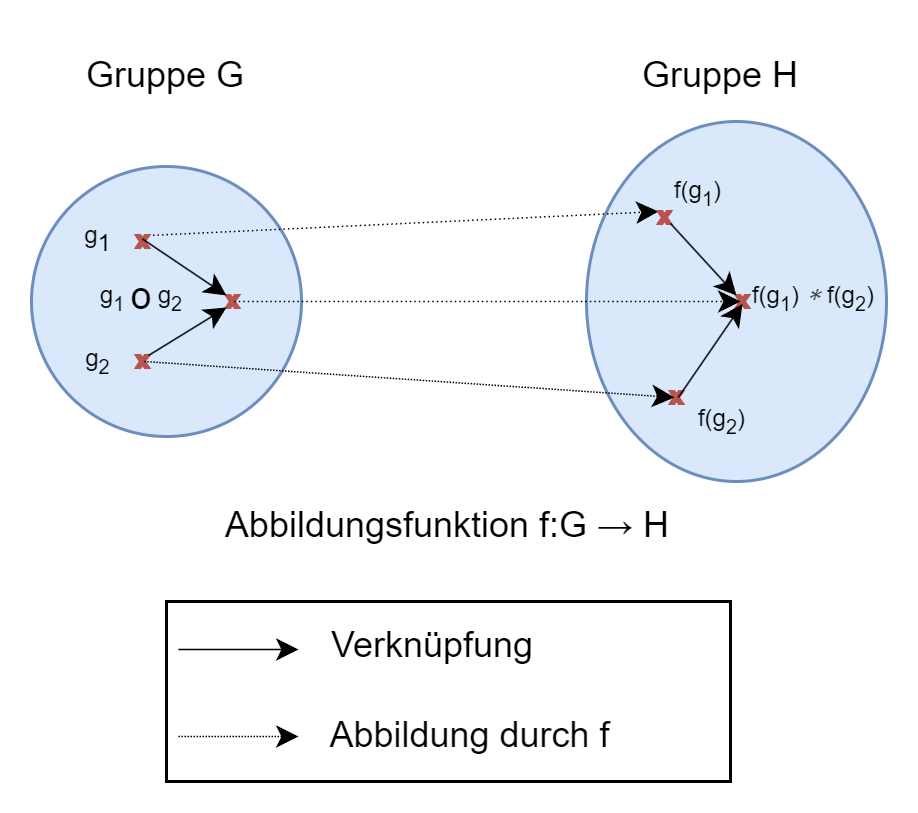
\includegraphics[width=12cm]{figures/group_homomophismus.png}
    \caption{Gruppenhomomorphismus nach \cite{P-98}}
    \label{fig:group_homomorphismus}
\end{figure} 

Bei der homomorphen Verschlüsselung, handelt es sich um einen Gruppenhomomorphismus zwischen der Gruppe der Klartexte $(P,\circ)$ und der Gruppe der Geheimtexte $(C,\ast)$. 
Die Abbildfunktionen sind dabei der Verschlüsselungsalgorithmus $Enc_k:P\to C$ und der Entschlüsselungsalgorithmus $Dec_k:C\to P$ mit einem Schlüssel $k \in K$ \cite{P-98}. 
Daraus lässt sich ableiten, dass folgende Bedingungen erfüllt sind:
\begin{equation*}
    Enc_k(p_1 \circ p_2) = Enc_k(p_1) \ast Enc_k(p_2) 
\end{equation*}
\begin{equation*}
Dec_k(c_1 \ast c_2) = Dec_k(c_1) \circ Dec_k(c_2)
\end{equation*}
Abbildung \ref{fig:homo_enc} zeigt, wie besagter Homomorphismus aussieht.


\begin{figure}[!htb]
    \centering
    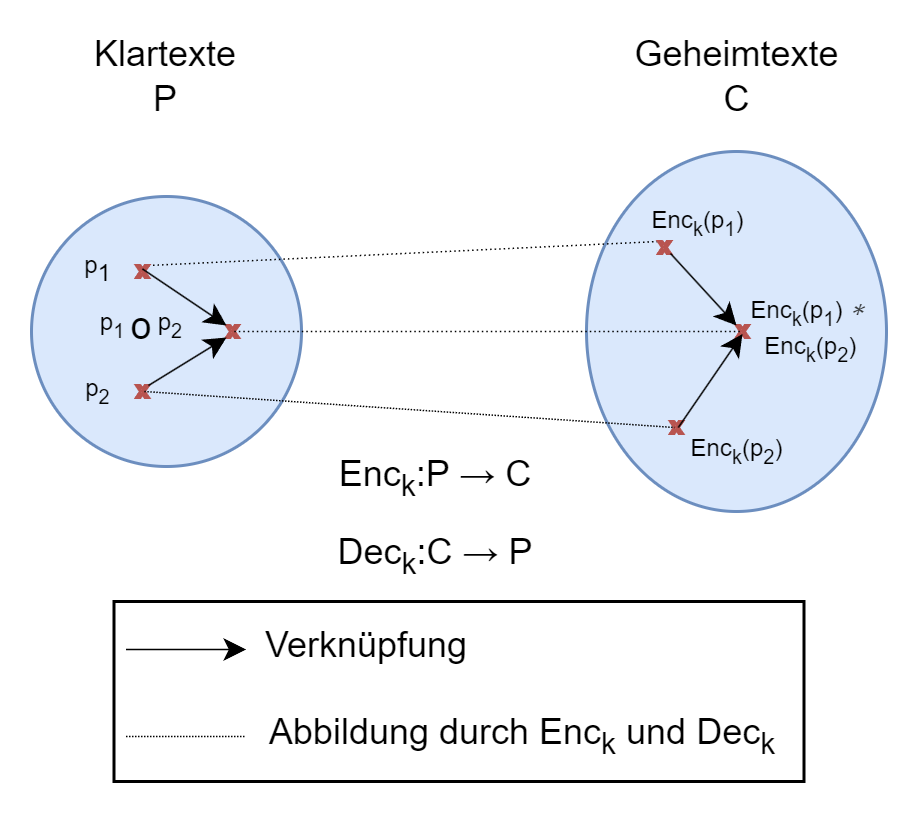
\includegraphics[width=12cm]{figures/homo_enc.png}
    \caption{Homomorphe Verschlüsselung}
    \label{fig:homo_enc}
\end{figure} 

Homomorphe Verschlüsselungen lassen sich dabei in 3 Kategorien einteilen, je nachdem welche Verknüpfungen innerhalb der Gruppen möglich sind \cite{P-42}:
\begin{compactitem}
\item \textbf{Teilweise homomorphe Verschlüsselung (partially):} Entweder Multiplikation oder Addition möglich, jedoch nicht beides.
\item \textbf{Eingeschränkte homomorphe Verschlüsselung (somewhat oder leveled):} Sowohl Multiplikation als auch Addition möglich, jedoch beschränkt durch die Anzahl an durchführbaren Berechnungen. 
\item \textbf{Vollständige homomorphe Verschlüsselung (fully):} Multiplikation und Addition für eine unbegrenzte Anzahl an Berechnungen möglich
\end{compactitem}

Gentry \cite{P-40} stellte 2009 das erste vollständig homomorphe Verschlüsselungssystem vor.
Dabei nutzte er eine eingeschränkt homomorphe Verschlüsselung, welche auf mathematischen Gittern basiert.
Das System war eingeschränkt homomorph, da die Verschlüsselung auf einem Rauschen basierte, welches mit jeder Operation größer wurde und letztendlich nicht mehr für eine korrekte Entschlüsselung sorgte.
Er erweiterte das System mit einer Technik namens Bootstrapping.
Dabei wird der Geheimtext ein zweites Mal verschlüsselt, sodass dieser doppelt verschlüsselt ist.
Anschließend kann mittels des verschlüsselten Schlüssels die ursprüngliche Verschlüsselung homomorph herausgerechnet werden. 
Dadurch wird das Rauschen des Verschlüsselungssystems zurückgesetzt und eine weitere Berechnung ist möglich. 
Kann das ursprünglich eingeschränkte homomorphe Verschlüsselungssystem die homomorphe Entschlüsselung und eine weitere Operation durchführen, dann kann es mittels Bootstrapping zu einem vollständig homomorphen Verschlüsselungssystem umgewandelt werden.
So nutzen beispielsweise Van Dijk et al. \cite{P-100} diesen Fakt aus, und ersetzten die auf Gittern basierte Verschlüsselung durch eine auf Ganzzahlen basierte, eingeschränkt homomorphe Verschlüsselung aus. 

Brakerski und Vaikuntanathan \cite{P-101} verbesserten die Effizienz des bereits geschilderten Ansatzes.
Sie nutzen eine eingeschränkte homomorphe Verschlüsselung auf Basis des Lernen mit Fehlern Problems (Learning with errors) zusätzlich zu einem Relinearisierungsschritt.
Dieser zusätzliche Relinearisierungsschritt reduziert die Größe des Geheimtextes, wodurch die homomorphe Entschlüsselung beim Bootstrapping vereinfacht wird.

Gentry et al. \cite{P-102} stellten eine weitere vollständig homomorphe Verschlüsselung auf Basis des Lernen mit Fehlern Problems vor.
Die darin eingesetzte, eingeschränkt homomorphe Verschlüsselung stellt den Geheimtext als eine Matrix dar.
Die Dimension der Matrix bleibt bei jeder homomorphen Operation gleich und wächst dadurch nicht.
Dies ermöglicht, den Relinearisierungsschritt zu entfernen.
Bei dem Bootstrapping bisheriger Algorithmen, musste der verschlüsselte Schlüssel oder der Public Key des Nutzers mitgeschickt werden.
Bei diesem Ansatz ist es jedoch möglich, alleine mit dem Geheimtext Operationen durchzuführen, die anschließend nur der Nutzer entschlüsseln kann.


Theoretisch wäre das Training eines Neuronalen Netzes mittels vollständiger homomorpher Verschlüsselung möglich, jedoch ist es nicht praktikabel. 
Das Training besteht aus vielen Berechnungsschritten (Inferenze, Berechnen der Verlustfunktion, Gradientenberechnung, Anpassen der Gewichte), welche mit der Größe des Neuronalen Netzes ansteigt.
So wird bereits bei einem Neuronales Netz mit 7 Schichten, Faltungsschichten und vollständig verbundene Schichten, die Trainingszeit auf einer gewöhnlichen CPU, von ungefähr einer Stunde auf ein ganzes Jahr erhöht \cite{P-103}.
Eine Alternative ist es, keine vollständige sondern nur eingeschränkte homomorphe Verschlüsselung zu nutzen.
Takabi et al. \cite{P-104} zeigen wie dies möglich ist.
Um das Problem der begrenzten Anzahl an Berechnungen von eingeschränkter homomorphen Verschlüsselung zu umgehen, wird ein zusätzlicher Schritt eingeführt. 
Wird das Rauschen der Verschlüsselung zu groß und überschreitet einen festgelegten Schwellenwert, muss der aktuelle Zustand entschlüsselt und neu verschlüsselt werden.
Hierdurch wird das Rauschen zurückgesetzt, ohne dass Bootstrapping nötig ist.
Dadurch, dass kein vollständig homomorphes Verschlüsselungssytem genutzt werden muss, können performantere, teilweise homomorphe Verschlüsselungssyteme genutzt werden.

Neben dem Training eines Modells, gibt es eine Vielzahl an Techniken, die Homomorphe Verschlüsselung nur bei der Inferenz der Neuronalen Netze nutzt. 
Diese werden in Kapitel \ref{sec:krypto_inferenz} genauer beschrieben.
Alternativ kann Homomorphe Verschlüsselung beim Verteilten Lernen eingesetzt werden, was in Kapitel \ref{sec:verteiltes_lernen} beleuchtet wird. 





\subsection{Funktionale Verschlüsselung}\label{sec:funktionale_verschlüsselung}

Eine weitere Methodik, Berechnungen auf verschlüsselten Daten durchzuführen, ist die sogenannte Funktionale Verschlüsselung.
Diese wurde 2011 von Boneh et al.\cite{P-44} vorgestellt.
Funktionale Verschlüsselung erlaubt es, eine Funktion $f$ eines Klartextes zu berechnen, wobei nur der Geheimtext als Input der Funktion genutzt wird.
Dies geschieht in vier Schritten\cite{P-44}:
\begin{compactenum}
    \item \textbf{Setup: } In einem Vorbereitungsschritt wird ein Public Key $pk$ und ein Master Secret Key $msk$ erzeugt.
    \begin{equation*}
        (pk, msk) \xleftarrow{} Setup
    \end{equation*}
    \item \textbf{Schlüsselgenerierung: } Der Master Secret Key kann nun genutzt werden, um einen spezifischen Secret Key $sk$ für eine definierte Funktion $f$ zu erzeugen.
    \begin{equation*}
        sk \xleftarrow{} Keygen(msk, f)
    \end{equation*}
    \item \textbf{Verschlüsselung: } Der Public Key $pk$ wird genutzt, um den Klartext $x$, auf welchem die Berechnung durchgeführt werden soll, zu verschlüsseln.
    \begin{equation*}
        c \xleftarrow{} Enc(pk,x)
    \end{equation*}
    \item \textbf{Entschlüsselung: } Die Entschlüsselung des Geheimtextes $c$ mittels des spezifischen Secret Key $sk$ entspricht hierbei der Berechnung der Funktion $f$ mit dem Parameter $x$.
    \begin{equation*}
        f(x) \xleftarrow{} Dec(sk,c)
    \end{equation*}
\end{compactenum}

Die ersten Ansätze um Funktionale Verschlüsselung und Neuronalen Netze zu verbinden, fokussierten sich auf die Inferenz der Modelle, welche in Kapitel \ref{sec:krypto_inferenz} genauer betrachtet werden.
Ein Framework für das Training des Modells mit dem Namen CryptoNN wurde jedoch von Xu et al. \cite{P-53} vorgestellt.
Dieses ermöglicht, ein Modell auf einem fremden Server (Cloud) zu trainieren, ohne dass der Provider Einblick in die Daten erhält.
Dabei wird eine Funktionale Verschlüsselung genutzt, welche die Berechnung des Skalarprodukts und zusätzlich auch die Grundrechenarten (Addition, Subtraktion, Multiplikation und Division) von zwei Vektoren elementweise ermöglicht.
Kombiniert ermöglicht dies, alle notwendigen Berechnungen beim Training des Modells durchzuführen.
CryptoNN führt dabei 3 Rollen ein: Autorität, Client und Server. 
Dabei ist es auch möglich, dass es mehrere Clients gibt, die zusammen ein Modell trainieren.
Gibt es jedoch nur einen Client, so übernimmt dieser auch die Rolle der Autorität.
Die Autorität ist dafür zuständig, einen Master Secret Key $msk$ und einen Public Key $pk$ zu erzeugen, den Public Key $pk$ an den Client zu verteilen und bei Bedarf spezifische Secret Keys $sk_n$ zu erzeugen und an den Server weiterzugeben.
Der Client ist Besitzer der Daten und verschlüsselt diese vor der Übergabe an den Server mit dem Public Key $pk$. 
Der Server führt das tatsächliche Training des Modells durch.
Beim Feedforward Schritt wird Funktionale Verschlüsselung zur Berechnung der Neuronen der ersten Hidden Layer genutzt.
Dafür fordert der Server einen spezifischen Secret Key $sk_n$ an, der die Berechnung der ersten Schicht ermöglicht.
Der restliche Feedforward Schritt erfolgt unverschlüsselt.
Wenn der Client auch das Label verschlüsselt, kann die Berechnung der Verlustfunktion für jedes Output Neuron ebenfalls verschlüsselt erfolgen.
Abbildung \ref{fig:cryptonn} zeigt das CryptoNN Framework.

\begin{figure}[!htb]
    \centering
    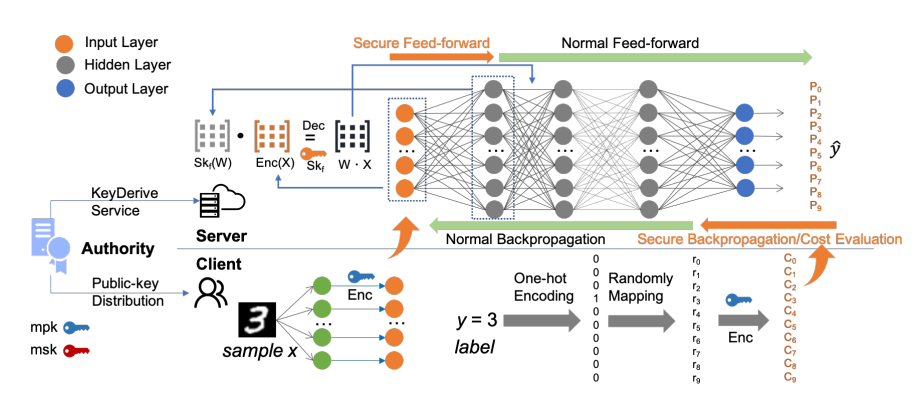
\includegraphics[width=15cm]{figures/cryptoNN}
    \caption{CryptoNN Framework \cite{P-53}}
    \label{fig:cryptonn}
\end{figure} 

Ein Problem des CryptoNN Frameworks ist jedoch, dass davon ausgegangen wird, dass der Server kein Angreifer ist, der effektiv versucht Daten zu extrahieren.
Ansonsten könnte dies dazu führen, dass der Server diverse White-Box Angriffe (Kapitel \ref{sec:angriffe}) durchführen könnte, da das Modell unverschlüsselt vorliegt.
Die Methodik ist demnach darauf ausgelegt dafür zu sorgen, dass Clients Daten verschlüsselt übertragen können und diese nicht beispielsweise von dem Cloud Provider mitgelesen werden können.


\subsection{Verteiltes Lernen}\label{sec:verteiltes_lernen}

Das Verteilte Lernen bietet einige besondere Herausforderungen, die bereits in Kapitel \ref{sec:angriffe_verteiltes_lernen} betrachtet wurden. 
Einige bereits beschriebene Methoden lassen sich problemlos auf das Verteilte Lernen anwenden.
Sollen beispielsweise die Daten der einzelnen Teilnehmer geteilt werden, so ist es möglich, diese mit den Methoden aus Kapitel \ref{sec:aufbereitung_datensatz} vorzuverarbeiten.
Jedoch gibt es auch spezielle Methoden, die auf das Verteilte Lernen ausgerichtet sind.
Im Folgenden werden einige davon genauer beschrieben.

\subsubsection*{Distributed Selective SGD}
Shokri und Shmatikov \cite{P-78} stellen eine Methode vor, bei welcher mehrere Teilnehmer gleichzeitig ein Modell trainieren, ohne dabei die Daten untereinander zu teilen.
Diese wird Distributed Selective Stochastic Gradient Descent oder auch Distributed Selective SGD genannt.
Das Modell liegt dabei auf einem zentralen Server.
Bei der ersten Iteration laden die Teilnehmer das gesamte Modell herunter, bei weiteren Iterationen nur eine festgelegte Anzahl der am meisten geupdateten Parametern (Gewichte).
Dadurch soll vermieden werden, dass Overfitting auf den Daten eines einzelnen Teilnehmers auftritt.
Die heruntergeladenen Parameter ersetzen die alten Parameter an der entsprechenden Stelle im lokalen Modell.
Anschließend wird dieses lokale Modell mit den eigenen Daten trainiert und im Nachhinein eine festgelegte Menge an Gradienten übertragen. 
Diese können dabei entweder randomisiert ausgewählt werden, oder möglichst nach Größe sortiert werden.
Alle Teilnehmer wählen die zu teilenden Gradienten mit der gleichen Strategie aus und behalten diese über den Trainingsprozess bei.
Zusätzlich ist es möglich, die Gradienten vor dem Teilen noch mit in der Größe zu begrenzen oder Rauschen mittels Differential Privacy hinzuzufügen.
Abbildung \ref{fig:dssgd} zeigt die Architektur von Distributed Selective SGD.

\begin{figure}[!htb]
    \centering
    \includegraphics[width=12cm]{figures/dssgd}
    \caption{Distributed Selective SGD \cite{P-78}}
    \label{fig:dssgd}
\end{figure} 

Durch das eingeschränkte Teilen der Gradienten werden so wenig Information wie nötig geteilt, jedoch ist die Güte des Modells kaum schlechter als bei normalem Training.
Die Autoren begründen dies damit, dass das lokale Modell lokale Minima durch das Ersetzen von Parametern aus dem geteilten Modell verlassen kann und so weiter eher Richtung globales Minimum konvergiert. 
Zwei Parameter steuern dabei die Performance des Modells beim Training mit Distributed Selective SGD: das Privacy Budget $\epsilon$ und die Anzahl der zu teilenden Gradienten.
Werden mehr Gradienten nach jedem Schritt von jedem Teilnehmer geteilt, kann das Privacy Budget $\epsilon$ niedriger angesetzt werden, um dennoch eine nahezu identische Güte im Vergleich zu einem normal trainierten Modell zu erhalten.

\subsubsection*{Anspruchsvolle kryptografische Methoden}

Takabi et al. \cite{P-104} nutzen Homomorphe Verschlüsselung, um ein Modell zu trainieren, welches Daten von mehreren Teilnehmern nutzen kann. 
Die Funktionsweise der Methode mit einem Teilnehmer wurde bereits in Kapitel \ref{sec:homomorphe_verschlüsselung} beschrieben.
Diese lässt sich problemlos auf mehrere Teilnehmer erweitern, indem abwechselnd Daten jedes Teilnehmers verschlüsselt an den Server übertragen wird und diese für das Training des Modells mittels Homomorpher Verschlüsselung genutzt wird.
Da Daten jeweils verschlüsselt sind, ist es nicht möglich, Daten anderer Teilnehmer zu extrahieren.

Auch das auf Funktionaler Verschlüsselung basierende Framework CryptoNN \cite{P-53}, welches in Kapitel \ref{sec:funktionale_verschlüsselung} vorgestellt wurde, kann für Verteiltes Lernen genutzt werden. 
Die Rolle des Clients können dabei mehrere Teilnehmer übernehmen, wohingegen die Autorität jedoch von einem separaten System übernommen werden muss. 
Anschließend können auch bei dieser Methode abwechselnd Daten von verschiedenen Teilnehmern zum Trainieren genutzt werden.

Ein weiterer Ansatz für Verteiltes Lernen, welches auf Funktionaler Verschlüsselung basiert, wurde von Xu et al. \cite{P-33} mit dem Namen HybridAlpha vorgestellt.
Ähnlich zu dem bereits beschriebenen CryptoNN Framework, gibt es auch eine Autorität, welche die benötigten kryptografischen Schlüssel an die Server und Clients verteilt.
Jedoch übertragen die Clients keine Daten an den Server, sondern trainieren ein lokales Modell.
Die aktualisierten Modellparameter werden anschließend mit Differential Privacy verrauscht und dann verschlüsselt an den Server übertragen.
Hat der Server alle verschlüsselten Modellparameter jedes Teilnehmers gesammelt, wird mittels Funktionaler Verschlüsselung die Summe der Gewichte jedes Neurons gebildet.
Daraus kann der Server anhand der Anzahl an Teilnehmern, den Durchschnittswert für jedes Gewicht jedes Neurons bilden und aktualisiert damit das globale Modell.
Die Autoren zeigen anhand des MNIST Datensatze \cite{D-MNIST}, dass die Güte eines Modells, welches mit HyrbidAlpha ohne Differential Privacy trainiert wurde, sehr nahe der Güte eines Modells ist, welches in einem Verteilten Lernen Szenario ohne HyrbidAlpha gelernt wurde. 
Wird jedoch zusätzlich Differential Privacy genutzt, sinkt die Güte des Modells. 
Mit einem Privacy Budget von $\epsilon=0,5$ sinkt die Genauigkeit der Klassifikation um knapp 10\%.


\subsubsection*{Secure Multi-Party Computation}

Bei der Secure Multi-Party Computation handelt es sich um einen Forschungsbereich mit dem Ziel, dass Teilnehmer gemeinsam eine Funktion berechnen können, ohne dass die einzelnen Eingabewerte aufgedeckt werden. 
Methoden dieses kryptografischen Forschungsgebiets können auch für Neuronale Netze genutzt werden.

Rouhani et al. \cite{P-71} stellten ein Framework namens DeepSecure vor, welches Oblivious Transfer, zu Deutsch vergessliche Übertragung, und Garbled Circuits, zu Deutsch verdrehte Schaltkreise, nutzt.
Oblivious Transfer ist ein kryptografisches Protokoll zwischen einem Sender und einem Empfänger, bei dem der Empfänger einen Index zwischen 1 und $n$ auswählt und der Sender die Nachricht mit dem entsprechenden Index übermittelt. 
Der Sender weiß dabei jedoch nicht, welcher Index ausgewählt wurde.
Diese Methodik wird auch 1-aus-$n$ Oblivious Transfer genannt.
Garbled Circuits, auch Yao's Garbled Circuits genannt, ist ebenfalls ein Protokoll, bei der eine Funktion als Boolescher Schaltkreis mit zwei Eingabegattern dargestellt wird.
Dabei erstellt einer der beiden Teilnehmer, hier Alice genannt, Wahrheitstabellen zu jedem Logikgatter des Schaltkreises. 
Die Inputs sind dabei nicht 0 und 1, sondern jeweils eine Folge von $k$ randomisierten Bits, welche 0 und 1 kodieren.
Die Ergebnisspalte dieser Wahrheitstabellen verschlüsselt Alice anschließend mit den beiden Inputs, sodass dies nur mit den beiden Inputs wieder entschlüsselt werden kann. 
Zusätzlich wird die Reihenfolge der Zeilen randomisiert, damit aufgrund der Reihenfolge keine Rückschlüsse gewonnen werden können. 
Dieser Schritt wird Garbling genannt und die entstandenen Tabellen sind sogenannte Garbled Tabellen.
Anschließend überträgt Alice die Garbled Tabellen an den zweiten Teilnehmer, hier Bob.
Mittels 1-aus-2 Oblivious Transfer wählt Bob eine von zwei Nachrichten aus, wobei der Index seinem Input entspricht und die zwei Nachrichten die kodierten Labels von Alice sind.
Die erhaltene Nachricht und das eigene Label können nun genutzt werden, um die Ergebnisspalte einer Garbled Tabelle zu entschlüsseln.
Bob führt dies für jedes Gatter des Schaltkreises aus.
Am Ende erhält Bob den Output des letzten Gatters, welchen jedoch einer der randomisierten Bitfolgen ist. 
Er übermittelt diesen an Alice und erhält dadurch den entsprechenden 0 oder 1 Wert.
DeepSecure wendet Garbled Circuits auf Neuronale Netze an.
Alice würde in diesem Fall die Daten besitzen und Bob das Modell, welches trainiert wird.
Der Feedforward Schritt würde dabei durch einen Booleschen Schaltkreis aus XOR und XNOR Gattern implementiert werden, wodurch die Berechnung der Vorhersage erfolgt.
Dadurch kann Bob den Wert der Verlustfunktion und anschließend der Gradienten bestimmen, ohne die Daten von Alice zu kennen.
Alice würde jedoch auch nicht die genauen Gewichte des Modells kennen.
Allerdings ist die Anzahl an benötigten Gattern, um ein Neuronales Netz darzustellen, enorm.
Einige Operationen, wie die Anwendung einer Aktivierungsfunktion, benötigt mehrere tausende Gatter.
Jedes dieser Gatter sorgt ebenfalls dafür, dass eine Menge an Daten übertragen werden muss.
Ein Neuronales Netz, welches $28\times28$ Pixel Bilder als Input nimmt, zwei Hidden Layers mit 300 und 100 Knoten (Sigmoid Aktivierungsfunktion) besitzt und eine Softmax Output Layer mit 10 Knoten hat, würde circa 171.300.000 Gatter ausmachen und in einem Feedforward Schritt ungefähr 2 Gigabyte an Daten übertragen.

\subsubsection*{Aggregation}
Eine alternative Methode wird von Bonawitz et al. \cite{P-36} vorgestellt.
Diese basiert auf sicherer Aggregation, welche mehrere Daten von unterschiedlichen Teilnehmern verbindet, ohne dass die Daten eines einzelnen Teilnehmers erkenntlich werden.
Teilnehmer trainieren ein lokales Modell mit den eigenen privaten Daten. 
Bevor die angepassten Parameter aber an das globale Modell übertragen werden, werden die Parameter mit den Parametern anderer Teilnehmer kryptografisch aggregiert.
Dadurch erhält das globale Modell Gradienten aller Trainingsdaten, ohne die einzelnen Daten zu kennen.

